\chapter{Le Montréal 3V2}
\label{montreal}

Nous allons ici présenter la solution sur laquelle nous nous appuyons pour réaliser notre propre radiogoniomètre à effet Doppler, le Montréal 3V2.
Pour réaliser cette documentation nous nous sommes appuyé sur la documentation trouvé sur le site f1lvt \cite{montreal}

\section{Évolution du Montréal}

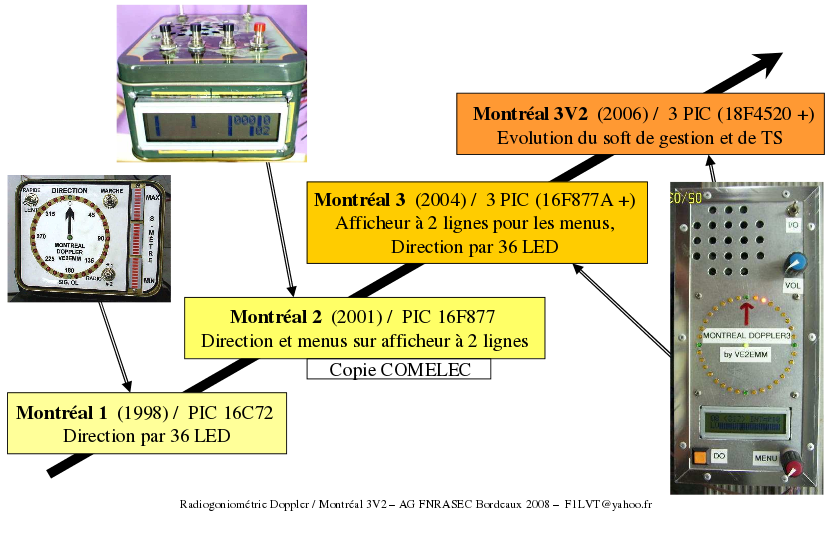
\includegraphics[width=\textwidth]{evolution}
\captionof{figure}{Evolution du Montréal}

\section{Avantages du Montréal 3v2}

\begin{center}
  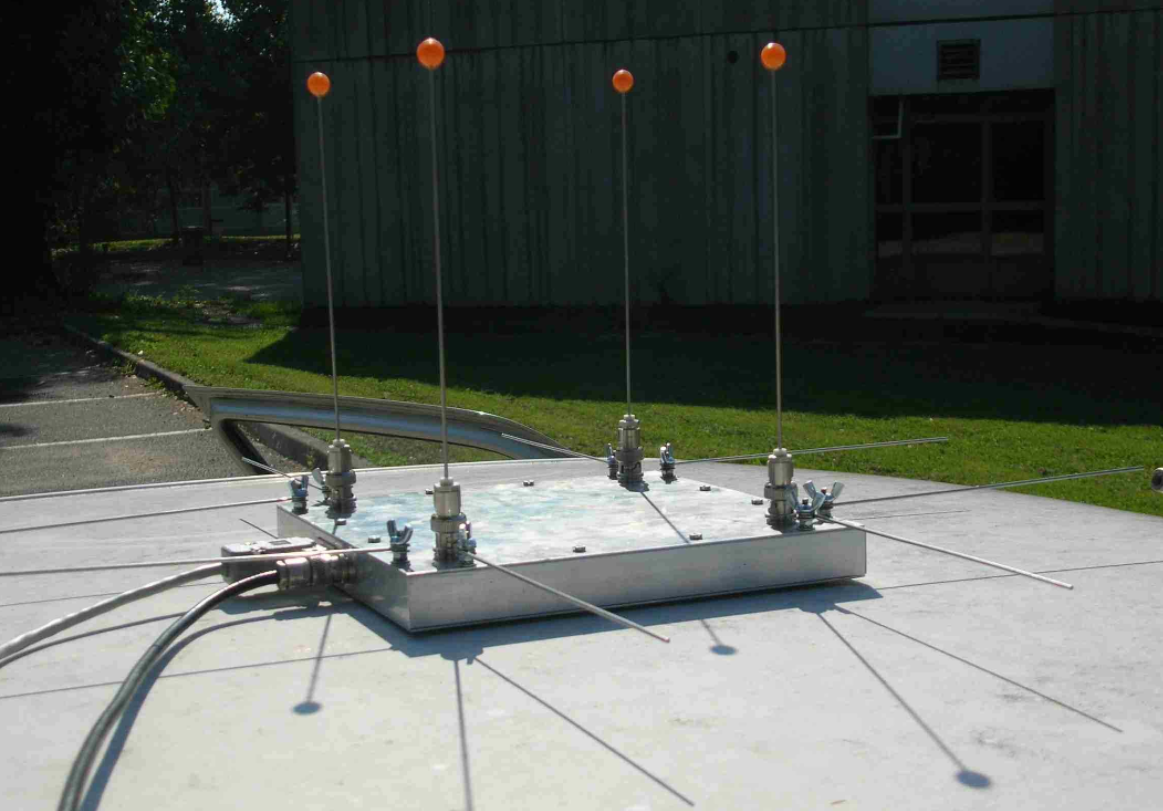
\includegraphics[width=0.5\textwidth]{montreal}
  \captionof{figure}{Photographie prise du Montréal 3v2}
\end{center}

Le Montréal 3v2 sert principalement à l'FNRASEC\footnote{Fédération Nationale des Radioamateurs au service de la Sécurité Civile, agrée de sécurité civile} et aux chasseurs d'onde amateurs. Ce radiogoniomètre est utilisé pour la détection de balise de détresse de 406MHz.

Parmi ses avantages, on peut noter qu'il est facile à construire, son prix de revient est très raisonnable, et il est simple d'utilisation. 

%on peut noter son affichage à 36 LED qui indique la direction de manière clair et efficace, et un réglage facilité par son écran LCD ou encore son filtre à capa commutée à très faible largeur de bande (0,5 Hz).

\section{Caractéristiques}

Le Montréal 3v2 est un radiogoniomètre à effet Doppler, il possède donc toutes les caractéristiques associé a ce type de radiogoniomètre.
~\\

\begin{tabular}{ l l l}
Fréquences & distance & moyenne portée\\
 & gamme & 50MHz-1.3GHz\\
 & démodulation & FM\\
Affichage & LED & 36LED\\
& écran & LCD en 2 lignes\\
Filtre & capa & très faible largeur de bande (0.5Hz)\\
Coût & & estimé à 50\euro \\
\end{tabular}



\section{Schéma bloc}

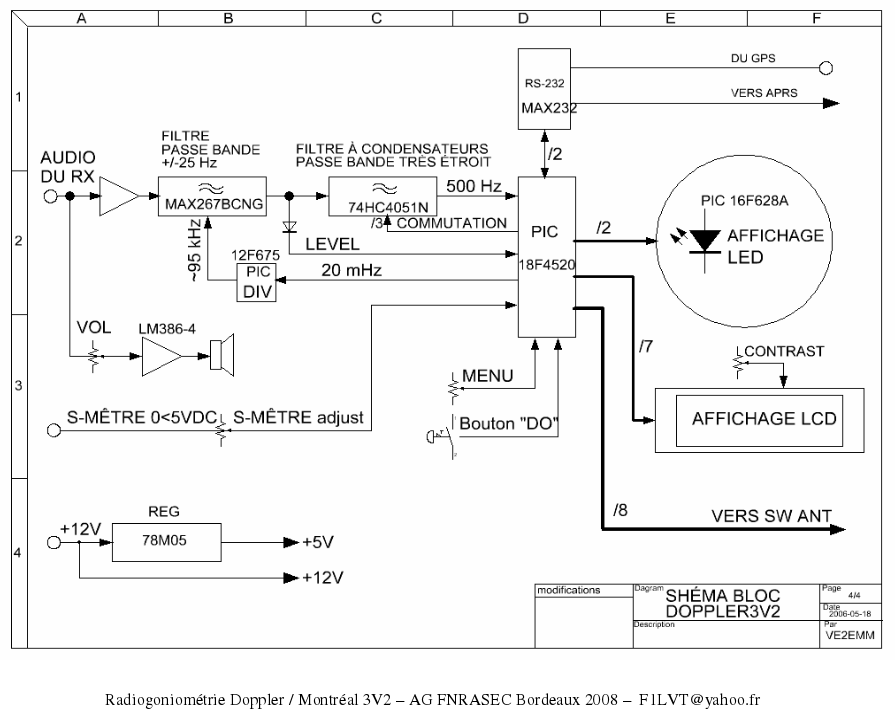
\includegraphics[width=\textwidth]{schemaBloc}
\captionof{figure}{Schéma bloc du Montréal 3v2}

\section{Liste des composants}
Voici la liste des composants pour la construction du Montréal 3v2:

\begin{tabular}{ l l l}

IC30&          LM386N-4&                  Ampli BF\\
IC50&          MAX267BCNG&          Filtre\\
IC51& PIC  12F675-I/P& PIC \\
IC52&          74HC4051N&               Filtre\\
IC53&          MAX492CPA &            Ampli Op\\
IC70& PIC  18F4520-I/P& PIC\\
VR20 &       7805 TO-220  &            Régulateur\\
X70&           20 MHz  HC49&           Quartz\\
D50&           1N5819       &                Diode Schottky\\
LCD20&      LCD 2X16,&                 Afficheur 2 lignes de 16 car.\\
IC1& PIC16F628A-I/P& PIC\\
LED1 - LED36& ø3mm, Rouge et/ou Vert&\\
LED37&                        3 ou 5mm Bicolore Rouge/Verte &\\
FB1 - FB8&                   Ferrites\footnote{+ composants passifs : Résistances, Condensateurs.}&\\
IC100&        = MAX232ACPE&        en option\\
Q100 &        = 2N2222 TO-92&\\
\end{tabular}



%%% Local Variables: 
%%% mode: latex
%%% TeX-master: "rapport_analyse"
%%% End: 
